%%%% 导言区
%% 设定纸张大小为A4, 基本字体大小为12pt, 文章题目单独为一页, 
%% 文档类型为article
\documentclass[12pt]{article}

%% en_preamble包含基本的宏包配置
%%%%%%%%------------------------------------------------------------------------
%%%% 日常所用宏包

%% 控制页边距
\usepackage[papersize={370mm,260mm},top=2cm, bottom=2cm, left=2.cm, right=2.cm,includefoot]{geometry}

%% 控制项目列表
\usepackage{enumerate}

%% 多栏显示
\usepackage{multicol}

%% hyperref宏包,生成可定位点击的超链接,并且会生成pdf书签
\usepackage[%
    pdfstartview=FitH,%
    CJKbookmarks=true,%
    bookmarks=true,%
    bookmarksnumbered=true,%
    bookmarksopen=true,%
    colorlinks=true,%
    citecolor=blue,%
    linkcolor=blue,%
    anchorcolor=green,%
    urlcolor=blue%
]{hyperref}

%% 控制标题
\usepackage{titlesec}

%% 控制表格样式
\usepackage{booktabs}

%% 控制目录
\usepackage{titletoc}

%% 控制字体大小
\usepackage{type1cm}

%% 首行缩进,用\noindent取消某段缩进
\usepackage{indentfirst}

%% 支持彩色文本、底色、文本框等
\usepackage{color,xcolor}

%% AMS LaTeX宏包
\usepackage{amsmath}

%% 一些特殊符号
% \usepackage{bbding}

%% 支持引用
% \usepackage{cite}

%% LaTeX一些特殊符号宏包
% \usepackage{latexsym}

%% 数学公式中的黑斜体
% \usepackage{bm}

%% 调整公式字体大小:\mathsmaller, \mathlarger
% \usepackage{relsize}

%% 生成索引
% \makeindex

%%%% 基本插图方法
%% 图形宏包
\usepackage{graphicx}

%% 多个图形并排,参加lnotes.pdf
\usepackage{subfig}

% \begin{figure}[htbp]               %% 控制插图位置
%   \setlength{\abovecaptionskip}{0pt}
%   \setlength{\belowcaptionskip}{10pt}
                                     %% 控制图形和上下文的距离
%   \centering                       %% 使图形居中显示
%   \includegraphics[width=0.8\textwidth]{CTeXLive2008.jpg}
                                     %% 控制图形显示宽度为0.8\textwidth
%   \caption{CTeXLive2008安装过程} \label{fig:CTeXLive2008}
                                     %% 图形题目和交叉引用标签
% \end{figure}
%%%% 基本插图方法结束

%%%% pgf/tikz绘图宏包设置
\usepackage{pgf,tikz}
\usetikzlibrary{shapes,automata,snakes,backgrounds,arrows}
\usetikzlibrary{mindmap}
%% 可以直接在latex文档中使用graphviz/dot语言,
%% 也可以用dot2tex工具将dot文件转换成tex文件再include进来
%% \usepackage[shell,pgf,outputdir={docgraphs/}]{dot2texi}
%%%% pgf/tikz设置结束


%%%% fancyhdr设置页眉页脚
%% 页眉页脚宏包
\usepackage{fancyhdr}

%% 页眉页脚风格
\pagestyle{plain}

%% 有时会出现\headheight too small的warning
\setlength{\headheight}{15pt}

%% 清空当前页眉页脚的默认设置
%\fancyhf{}
%%%% fancyhdr设置结束


%%%% 设置listings宏包用来粘贴源代码
%% 方便粘贴源代码,部分代码高亮功能
\usepackage{listings}

%% 所要粘贴代码的编程语言
\lstloadlanguages{}

%% 设置listings宏包的一些全局样式
%% 参考http://hi.baidu.com/shawpinlee/blog/item/9ec431cbae28e41cbe09e6e4.html
\lstset{
showstringspaces=false,              %% 设定是否显示代码之间的空格符号
numbers=left,                        %% 在左边显示行号
numberstyle=\tiny,                   %% 设定行号字体的大小
basicstyle=\footnotesize,                    %% 设定字体大小\tiny, \small, \Large等等
keywordstyle=\color{blue!70}, commentstyle=\color{red!50!green!50!blue!50},
                                     %% 关键字高亮
frame=shadowbox,                     %% 给代码加框
rulesepcolor=\color{red!20!green!20!blue!20},
escapechar=`,                        %% 中文逃逸字符,用于中英混排
xleftmargin=2em,xrightmargin=2em, aboveskip=1em,
breaklines,                          %% 这条命令可以让LaTeX自动将长的代码行换行排版
extendedchars=false                  %% 这一条命令可以解决代码跨页时,章节标题,页眉等汉字不显示的问题
}
%%%% listings宏包设置结束


%%%% 附录设置
\usepackage[title,titletoc,header]{appendix}
%%%% 附录设置结束


%%%% 日常宏包设置结束
%%%%%%%%------------------------------------------------------------------------

%%%%%%%%------------------------------------------------------------------------
%%%% 英文字体设置结束
%% 这里可以加入自己的英文字体设置
%%%%%%%%------------------------------------------------------------------------

%%%%%%%%------------------------------------------------------------------------
%%%% 设置常用字体字号,与MS Word相对应

%% 一号, 1.4倍行距
\newcommand{\yihao}{\fontsize{26pt}{36pt}\selectfont}
%% 二号, 1.25倍行距
\newcommand{\erhao}{\fontsize{22pt}{28pt}\selectfont}
%% 小二, 单倍行距
\newcommand{\xiaoer}{\fontsize{18pt}{18pt}\selectfont}
%% 三号, 1.5倍行距
\newcommand{\sanhao}{\fontsize{16pt}{24pt}\selectfont}
%% 小三, 1.5倍行距
\newcommand{\xiaosan}{\fontsize{15pt}{22pt}\selectfont}
%% 四号, 1.5倍行距
\newcommand{\sihao}{\fontsize{14pt}{21pt}\selectfont}
%% 半四, 1.5倍行距
\newcommand{\bansi}{\fontsize{13pt}{19.5pt}\selectfont}
%% 小四, 1.5倍行距
\newcommand{\xiaosi}{\fontsize{12pt}{18pt}\selectfont}
%% 大五, 单倍行距
\newcommand{\dawu}{\fontsize{11pt}{11pt}\selectfont}
%% 五号, 单倍行距
\newcommand{\wuhao}{\fontsize{10.5pt}{10.5pt}\selectfont}
%%%%%%%%------------------------------------------------------------------------


%%%%%%%%------------------------------------------------------------------------
%%%% 一些个性设置

%% 设定页码方式,包括arabic、roman等方式
%% \pagenumbering{arabic}

%% 有时LaTeX无从断行,产生overfull的错误,这条命令降低LaTeX断行标准
%% \sloppy

%% 设定目录显示深度\tableofcontents
%% \setcounter{tocdepth}{2}
%% 设定\listoftables显示深度
%% \setcounter{lotdepth}{2}
%% 设定\listoffigures显示深度
%% \setcounter{lofdepth}{2}

%% 设定段间距
\setlength{\parskip}{0.3\baselineskip}

%% 设定行距
\linespread{1}

%% 中文破折号,据说来自清华模板
\newcommand{\pozhehao}{\kern0.3ex\rule[0.8ex]{2em}{0.1ex}\kern0.3ex}

%% 设定itemize环境item的符号
\renewcommand{\labelitemi}{$\bullet$}

%% 设定正文字体大小
% \renewcommand{\normalsize}{\sihao}

%%%% 个性设置结束
%%%%%%%%------------------------------------------------------------------------


%%%%%%%%------------------------------------------------------------------------
%%%% bibtex设置

%% 设定参考文献显示风格
\bibliographystyle{unsrt}

%%%% bibtex设置结束
%%%%%%%%------------------------------------------------------------------------


%% 如果不写中文的话就不需要引用xecjk_preamble里面的配置
%%%%%%%%------------------------------------------------------------------------
%%%% xeCJK相关宏包

\usepackage{xltxtra,fontspec,xunicode}

%% \CJKsetecglue{\hskip 0.15em plus 0.05em minus 0.05em}
%% slanfont: 允许斜体
%% boldfont: 允许粗体
%% CJKnormalspaces: 仅忽略汉字之间的空白,但保留中英文之间的空白。 
%% CJKchecksingle: 避免单个汉字单独占一行。
\usepackage[slantfont, boldfont]{xeCJK} 

%% 针对中文进行断行
\XeTeXlinebreaklocale "zh"             

%% 给予TeX断行一定自由度
\XeTeXlinebreakskip = 0pt plus 1pt minus 0.1pt

%%%% xeCJK设置结束                                       
%%%%%%%%------------------------------------------------------------------------

%%%%%%%%------------------------------------------------------------------------
%%%% xeCJK字体设置

%% 设置中文标点样式,支持quanjiao、banjiao、kaiming等多种方式
\punctstyle{kaiming}                                        
                                                     
%% 设置缺省中文字体
\setCJKmainfont[BoldFont={simhei.ttf}, ItalicFont={simkai.ttf}]{simsun.ttc}   
%% 设置中文无衬线字体
\setCJKsansfont[BoldFont={simhei.ttf}]{simkai.ttf}  
%% 设置等宽字体
\setCJKmonofont{simhei.ttf}                            

%% 英文衬线字体
\setmainfont{DejaVu Serif}                                  
%% 英文等宽字体
\setmonofont{DejaVu Sans Mono}                              
%% 英文无衬线字体
\setsansfont{DejaVu Sans}                                   

%% 定义新字体
\setCJKfamilyfont{song}{simsun.ttc}                     
\setCJKfamilyfont{kai}{simkai.ttf}
\setCJKfamilyfont{hei}{simhei.ttf}
\setCJKfamilyfont{fangsong}{simfang.ttf}
%\setCJKfamilyfont{lisu}{LiSu}
%\setCJKfamilyfont{youyuan}{YouYuan}

%% 自定义宋体
\newcommand{\song}{\CJKfamily{song}}                       
%% 自定义楷体
\newcommand{\kai}{\CJKfamily{kai}}                         
%% 自定义黑体
\newcommand{\hei}{\CJKfamily{hei}}                         
%% 自定义仿宋体
\newcommand{\fangsong}{\CJKfamily{fangsong}}               
%% 自定义隶书
%\newcommand{\lisu}{\CJKfamily{lisu}}                       
%% 自定义幼圆
%\newcommand{\youyuan}{\CJKfamily{youyuan}}                 

%%%% xeCJK字体设置结束
%%%%%%%%------------------------------------------------------------------------

%%%%%%%%------------------------------------------------------------------------
%%%% 一些关于中文文档的重定义

%% 数学公式定理的重定义

\newtheorem{example}{例}                                   
\newtheorem{algorithm}{算法}
%% 按section编号
\newtheorem{theorem}{定理}[section]                         
\newtheorem{definition}{定义}
\newtheorem{axiom}{公理}
\newtheorem{property}{性质}
\newtheorem{proposition}{命题}
\newtheorem{lemma}{引理}
\newtheorem{corollary}{推论}
\newtheorem{remark}{注解}
\newtheorem{condition}{条件}
\newtheorem{conclusion}{结论}
\newtheorem{assumption}{假设}

%% 章节等名称重定义
\renewcommand{\contentsname}{目\hspace{1.5cm}录}     
\renewcommand{\abstractname}{摘要}
\renewcommand{\indexname}{索引}
\renewcommand{\listfigurename}{插图目录}
\renewcommand{\listtablename}{表格目录}
\renewcommand{\figurename}{图}
\renewcommand{\tablename}{表}
\renewcommand{\appendixname}{附录}
\renewcommand{\appendixpagename}{附录}
\renewcommand{\appendixtocname}{附录}
\renewcommand\refname{参考文献} 

%% 设置chapter、section与subsection的格式
\titleformat{\chapter}{\centering\huge}{第\thechapter{}章}{1em}{\textbf}
%\titleformat{\section}{\centering\sanhao}{\hei \biaotiNR\thesection}{1em}{\textbf}
%\titleformat{\subsection}{\xiaosi}{\thesubsection}{1em}{\textbf}
%\titleformat{\subsubsection}{\xiaosi}{\thesubsubsection}{1em}{\textbf}

\usepackage{listings}

%%%% 中文重定义结束
%%%%%%%%------------------------------------------------------------------------


\usepackage{tabu} % 用tabu代替 array
\usepackage{multirow}
\usepackage{zhnumber}
\usepackage{calc,marvosym,ifthen,fancybox,url,layout}

\newcolumntype{M}[1]{>{\sihao\centering\arraybackslash}m{#1}}
\newcolumntype{N}{@{}m{0pt}@{}}

\setlength{\parindent}{0pt}

%% 首页格式
%\usepackage{tabu} % 用tabu代替 array
\usepackage{multirow}
\usepackage{zhnumber}
\usepackage{calc,marvosym,ifthen,fancybox,url,layout}
\setcounter{tocdepth}{1}

%设定标题
\setcounter{secnumdepth}{5}
\titleformat{\section}{\centering\sanhao}{\hei \biaotiNR\thesection}{1em}{\hei}
\titleformat{\subsection}{\xiaosi}{\hskip -2pt \Roman{subsection}}{1em}{\hei}
\titleformat{\subsubsection}{\xiaosi}{\hei\zhnumber{\arabic{subsubsection}}、}{1em}{\textbf}
\titleformat{\paragraph}{\xiaosi}{\arabic{paragraph}、}{1em}{}
\titleformat{\subparagraph}{\xiaosi}{(\arabic{subparagraph})}{1em}{}
%调整标题间距
\titlespacing{\subsection}{0pt}{*0}{*0}
\titlespacing{\subsubsection}{0pt}{*0}{*0}
\titlespacing{\section}{0pt}{*0}{*0}
\titlespacing{\paragraph}{0pt}{*0}{*0}
\titlespacing{\subparagraph}{0pt}{*0}{*0}
 
 %给旁注加个黑原点
\usepackage{wasysym}
\let\marginparNR\marginpar
\def\marginpar#1{\marginparNR{ \CIRCLE{}   #1  }}

%调整列表前后的间距
\makeatletter
\let\orig@Enumerate=\enumerate
\renewenvironment{enumerate}{\orig@Enumerate}{\vspace{-0.5cm}\endlist}
\let\orig@Itemize=\itemize
\renewenvironment{itemize}{\orig@Itemize}{\vspace{-0.5cm}\endlist}
\makeatother

%给目录进行设定
\titlecontents{section}[0pt]{\addvspace{5pt}\filright}
{\biaotiNR {\thecontentslabel\ } \hspace{0.5em} }
{}{\titlerule*[8pt]{.}\contentspage}


%画边框
%\def\boxhack{\leavevmode\vbox to0pt{\vss\rlap{\hskip 320pt
%			\setlength{\unitlength}{1pt}\cornersize*{10pt}\thicklines\fancyoval(365,675)}\vskip -680pt}}
%\def\boxhackb{\leavevmode\vbox to0pt{\vss\rlap{\hskip 80pt
%			\setlength{\unitlength}{1pt}\cornersize*{10pt}\thicklines\fancyoval(100,675)}\vskip -680pt}}

%用tikz画边框	
\def\biankuang{\leavevmode\vbox to0pt{
		\vss\rlap{\hskip 0.8cm
			\tikz \draw(4,0)--(0,0)--(0,-23.7)--(16.7,-23.7)--(16.7,0)--(4,0)--(4,-23.7);		
		}\vskip -24cm}}
		
\newcolumntype{M}[1]{>{\sihao\centering\arraybackslash}m{#1}}
\newcolumntype{N}{@{}m{0pt}@{}}

\newcommand{\ktmq}[1]{\gdef\ktmqNR{#1}}%课题名称
\newcommand{\jxmb}[1]{\gdef\jxmbNR{#1}}%教学目标
\newcommand{\jxnd}[1]{\gdef\jxndNR{#1}}%教学难点
\newcommand{\jxzd}[1]{\gdef\jxzdNR{#1}}%教学重点
\newcommand{\jjff}[1]{\gdef\jjffNR{#1}}%解决方法
\newcommand{\jxhj}[1]{\gdef\jxhjNR{#1}}%教学后记

\newcommand{\jc}[1]{\gdef\jcNR{#1}}%教材
\newcommand{\cks}[1]{\gdef\cksNR{#1}}%参考书
\newcommand{\jsxm}[1]{\gdef\jsxmNR{#1}}%教师姓名
\newcommand{\jyszr}[1]{\gdef\jyszrNR{#1}}%教研室主任

\newcommand{\skbc}[1]{\gdef\skbcNR{#1}}%授课班次
\newcommand{\skrq}[1]{\gdef\skrqNR{#1}}%授课日期
\newcommand{\biaoti}[1]{\gdef\biaotiNR{#1}}%标题头

\newcounter{thesectionSY}

\newcommand{\makeshouye}{
	\setcounter{thesectionSY}{\thesection+1}
	\restoregeometry	
	\renewcommand{\headrulewidth}{0pt}
	\pagestyle{fancy}
	\fancyhead{}
	\lhead{} 
	\chead{
		\begin{tabular}{@{\hspace{1.2cm}}M{7cm}@{\hspace{-0.4cm}}M{8cm}N}
			\parbox{7cm}{\linespread{0.2}
				\makebox[7cm][s]{\kai \sanhao 湖南九嶷职业技术学院}\\ 
				\makebox[7cm][s]{\kai \sanhao 湖南潇湘技师学院}
			}
			&  \makebox[6cm][s]{\rule{0pt}{0.9cm}\yihao \hei 授课课时计划}\\
		\end{tabular}
	}
	
	\begin{tabular}{M{2.2cm}|M{7cm}|M{5.8cm}N}
		\hline
		\multirow{2}*{
			\rule{0pt}{1.4cm}\parbox[b]{2.cm}{
				\centering 课\hfill 程\hfill 章\hfill 节\\及\hfill 主\hfill 题}}& \hei \biaotiNR\thethesectionSY  &  ~授~课~教~师\hfill {\kai \sanhao \underline{\jsxmNR}}\hfill 签字~~~&\\[0.6cm] \cline{2-3}
		
		& \hei \ktmqNR &  ~教研室主任\hfill {\fangsong \sanhao \underline{\jyszrNR}}\hfill 签字~~~&\\[0.6cm]\hline
		
		\multicolumn{3}{l}{
			\begin{minipage}[t][4cm][t]{15cm}	
				\begin{minipage}[t]{2.5cm}
					\vspace{6pt} \hfill \sihao 教学目标:
				\end{minipage}\hspace{0.5cm}				
				\begin{minipage}[t][4cm][t]{12cm}
					\vspace{0pt}\sihao \setlength{\baselineskip}{12pt} 
					\begin{enumerate}[1、]
						\jxmbNR
					\end{enumerate} 
				\end{minipage} 
			\end{minipage}
		}\vspace{0.3cm} &\\ \hline
		\multicolumn{3}{l}{
			\begin{minipage}[t][6.5cm][t]{15cm}
				\begin{minipage}[t]{2.5cm}
					\vspace{5pt} \hfill \sihao 教学重点:
				\end{minipage}\hspace{0.5cm}				
				\begin{minipage}[t]{12cm}
					\vspace{0pt} \sihao \setlength{\baselineskip}{12pt} 
					\begin{enumerate}[1、] \jxzdNR \end{enumerate}
					\vspace{7pt} 
				\end{minipage}
				\vspace{5pt} 
				\begin{minipage}[t]{2.5cm}
					\vspace{6pt} \hfill \sihao 教学难点:
				\end{minipage}\hspace{0.5cm}		
				\begin{minipage}[t]{12cm}
					\vspace{0pt} \sihao \setlength{\baselineskip}{12pt} 
					\begin{enumerate}[1、] \jxndNR \end{enumerate}
					\vspace{0pt} 	
				\end{minipage}
				\begin{minipage}[t]{2.5cm}
					\vspace{6pt} \hfill \sihao 解决方法:
				\end{minipage}\hspace{0.5cm}		
				\begin{minipage}[t]{12cm}
					\vspace{6pt}\sihao \jjffNR
				\end{minipage}
				
			\end{minipage}
		} &\\  \hline
		
		\multirow{2}*{ 	\rule{0pt}{1.4cm}\parbox[b]{2.cm}{
				\centering 教\hfill 材\hfill 和\\参\hfill 考\hfill 书 } } & \multicolumn{2}{c}{\sihao \jcNR } &\\[0.6cm] \cline{2-3}
		&  \multicolumn{2}{c}{\sihao \cksNR } &\\[0.6cm] \hline
		\multirow{2}*{\rule{0pt}{1.4cm}\parbox[b]{2.cm}{
				\centering 授\hfill 课\hfill 班\hfill 次\\授\hfill 课\hfill 日\hfill 期 } } & \multicolumn{2}{c}{ \skbcNR } &\\[0.6cm] \cline{2-3}
		&\multicolumn{2}{c}{ \skrqNR } &\\[0.6cm] \hline
		
		\multicolumn{3}{l}{
			\begin{minipage}[t]{2.5cm}
				\vspace{0pt} \hfill \sihao 教学后记:
			\end{minipage}\hspace{0.5cm}				
			\begin{minipage}[t][4.5cm][t]{12cm}
				\vspace{0pt}\sihao \jxhjNR
			\end{minipage} 
		}\vspace{0.3cm} &\\ \hline	
	\end{tabular}
	\newpage
\newgeometry{textwidth={\textwidth-150pt},top=2cm,bottom=2cm,right=2.5cm,includehead,includefoot,marginparsep=28pt,marginparwidth=85pt}
	
\reversemarginpar
\fancyhead{} 
\chead{\kai \yihao 教 \hspace{1cm} 案 \hspace{1cm} 纸 }
%\lhead{\boxhack \boxhackb } %边框 
\lhead{ \biankuang}%边框 
		
\section{ \ktmqNR }
}



%%%% 导言区结束
%%%%%%%%------------------------------------------------------------------------

%%%%%%%%------------------------------------------------------------------------

%%%% 正文部分
\begin{document}
\setlength{\columnsep}{30pt } 
\columnseprule=0pt \twocolumn

\begin{center}
 \begin{tabular}{M{12em}M{4cm}N}
	\parbox{12em}{ \linespread{0.2}\xiaosi \bf \song	
		\makebox[12em][s]{湖南九嶷职业技术学院}\\[0.1cm]
		\makebox[12em][s]{湖南潇湘技师学院}
	}
	&  \yihao \hei \makebox[4cm][s]{\rule{0pt}{0.9cm}授课计划}&\\
\end{tabular}
\vspace{0.8cm}

\sanhao \bf  \underline{~~~2016--2017~~~} 学年  \underline{~~~2~~~}  学期
\end{center}

 \begin{tabular}{Nllll}
&系部:\underline{\makebox[12em]{\textbf{机电工程系}}}& 
专业: \underline{\makebox[7em]{\textbf{数控技术}}}&
班级: \underline{\makebox[9em]{\textbf{13级5年大专班}}}& \\[2ex]
&课程:\underline{\makebox[12em]{\textbf{《数控编程与实习》}}}&
上课周数:\underline{\makebox[5em]{\textbf{17}}} &
周学时:  \underline{\makebox[8em]{\textbf{[4](3)}}} & 
\end{tabular}
\vspace{0.3ex}

 {\bf 本学期课时分配表}
\vspace{0.ex}

%\hspace{-0.5em}
\begin{tabular}{|M{4em}|M{2.5em}|M{2.5em}|M{2.5em}|M{2.5em}|M{2.5em}|M{2.5em}|M{2.5em}|M{2.5em}|M{3em}|N}
	\hline 
	教学\par 模式 & \multicolumn{2}{c|}{理论}& \multicolumn{2}{c|}{一体化} & \multicolumn{2}{c|}{实习}&  \multirow{3}{*}{考}& \multirow{3}{*}{机}  &
	 \multirow{3}{*}{合} & \\[4.5ex]
	\cline{1-7} 
	教学 \par  形式& 讲\par  课 & 实\par  验 & 理\par 论\par 讲\par 课& 实\vspace{5.5ex} 训 & 理\par 论\par 讲\par 课 & 生\par 产\par 实\par 习 &\multirow{3}{*}{核}&\multirow{3}{*}{动}&\multirow{3}{*}{计}&\\ [12ex]
	\hline 
	 课时&×&×&0&\wuhao [64](48)&×&×&0&\wuhao [3](3)&\wuhao [68](51)& \\[4ex]
	\hline 
\end{tabular} 

~\vspace{0.3ex}

 说明:与本课程无关教学模式的各项各打×
\vspace{0.5ex}

 备注:~~
\begin{minipage}[t]{15cm}\vspace{-1.25em}
\begin{enumerate}[1、]
	\item 本课程以前完成学时数:\underline{\makebox[22em]{\textbf{0}}}
	\item 本课程在以后学期尚余留时数:\underline{\makebox[19em]{\textbf{32(180)  }}}        
	\item 本课程本学期列为考试(考查)课程:\underline{\makebox[16.8em]{\textbf{理论考试(实习考查)  }}} 
	\item 本课程使用教材名称: \underline{\makebox[23em]{\textbf{数控机床编程与操作(数控铣床~加工中心分册)}}}
\end{enumerate}
\end{minipage}
\vspace{0.5ex}

\newcommand{\ud}[2]{\underline{\makebox[#1]{\textbf{#2}}} }
\setlength{\baselineskip}{1.5\baselineskip}
\makebox[5em][s]{任课教师}:\ud{10em}{}  \hspace{1em} 编写日期:\ud{5.5em}{}年\ud{3em}{}月\ud{3em}{}日\\
\makebox[5em][s]{教研室主任}:\ud{10em}{}  \hspace{1em} 编写日期:\ud{5.5em}{}年\ud{3em}{}月\ud{3em}{}日\\
\makebox[5em][s]{系主任}:\ud{10em}{}  \hspace{1em} 编写日期:\ud{5.5em}{}年\ud{3em}{}月\ud{3em}{}日\\
\makebox[5em][s]{教务处}:\ud{10em}{}  \hspace{1em} 编写日期:\ud{5.5em}{}年\ud{3em}{}月\ud{3em}{}日\\
\makebox[5em][s]{分管领导}:\ud{10em}{}  \hspace{1em} 编写日期:\ud{5.5em}{}年\ud{3em}{}月\ud{3em}{}日\\

\pagebreak

\begin{center}
\erhao \hei 学期授课计划说明
\end{center}
\xiaosi \setlength{\parindent}{2em} \setlength{\baselineskip}{22pt}

\textbf{一、教学目的与要求:}

本学期主要在上个学期的基础上学习数控编程中的手工编程,要求学生能熟练运用各种编程方法来解决实际问题,充分把自己的能力及智慧通过编程展示出来。为以后走上工作岗位作好准备。

\textbf{二、用教材、参考书(书名、作者、出版社)}

1、使用教材: 《数控机床编程与操作(数控铣床 加工中心分册)》 沈建峰

2、参考书:《加工中心编程与操作》  科学出版社  刘加孝   主编

\hspace{4.5em}《加工中心操作工》 中国劳动社会保障出版社  杨伟群  主编

\hspace{4.5em}《加工中心考工实训教程》  化学工业出版社   吴明友 主编

\textbf{三、教学措施}

1、采用多媒体、仿真、讨论等教学方法。

2、作业:理论课每周布置一道编程题,仿真每周做习题集上的题目,实习除了完成课题外,还要每个课题写一个实习报告。
3、学生评价采用自评、小组评价、教师评价三结合。

\textbf{四、增删内容}

本计划无增删内容。

\textbf{五、本课程与其他课程的关系}

本课程是专业课,其他课程是基础,为本课服务。先要学习好《数控加工工艺》、《普铣》、《机械制图》、《机械加工原理》、《专业数学》等课程。在这些课程的基础上再来学习本课程就容易多了,希望同学们多复习这些课程。

\textbf{六、课程计划周数:}

授课时间为2\~{}18周(第1周教师备课、学生生报到注册,第19周考试),周课时8节。

\newpage 
\onecolumn \setlength{\parindent}{0em}
%
%\begin{center}
%	\begin{tabular}{M{12em}M{4cm}N}
%		\parbox{12em}{\linespread{0.2} 
%			\xiaosi \bf \song	\makebox[12em][s]{湖南九嶷职业技术学院}\\[0.1cm]
%			\makebox[12em][s]{湖南潇湘技师学院}
%		}
%		&  \yihao \hei \makebox[8cm][s]{\rule{0pt}{0.9cm}教师学期授课计划}&\\
%	\end{tabular}
%\end{center}
% 
%\newcolumntype{M}[1]{>{\xiaosan\arraybackslash}m{#1}}
%\begin{tabular}{|>{\centering}M{1.5cm}|M{6cm}|M{9cm}|>{\centering}M{4cm}|>{\centering}M{5cm}|>{\centering}M{2cm}|>{\centering}M{2.5cm}|N}
% 	\hline 
% 周次&\centering 授课章节内容摘要&\centering 教学 要求& 教具及实验\par 实习材料& 作业及参考材料& 教学\par 时数& 备注& \\[4.5ex] \hline
%1& 教师报到、学生报到 		& & & & & 02.13 02.19 & \\[4.5ex] \hline
%2& 理论1、复习导入 & 复习上学期所学内容&自绘示意图1&习题1& 2节 & 02.20 02.26 &  \\[4.5ex] \hline
%3& 理论2、变量编程概述 &掌握变量及用变量来编程 &自绘示意图2&习题2 & 2节 & 02.27 03.05 & \\[4.5ex] \hline
%4& 理论3、变量Z向分层 &掌握Z向分层的应用 &自绘示意图3&习题3 &2节 & 03.06 03.12 & \\[4.5ex] \hline
%5& 理论4、椭圆编程	&掌握椭圆加工及while指令 &自绘示意图4&习题4 & 2节& 03.13 03.19 & \\[4.5ex] \hline
%6& 理论5、椭圆弧编程 	& 掌握椭圆弧的加工&自绘示意图5 &习题5 &2节 & 03.20 03.26 & \\[4.5ex] \hline
%7& 理论6、局部坐标系 & 掌握局部坐标系的使用& 自绘示意图6&习题6 & 2节& 03.27 04.02 & \\[4.5ex] \hline
%8& 理论7、坐标系旋转(一) &掌握坐标系旋转的使用 & 自绘示意图7&习题7 & 2节& 04.03 04.09 & \\[4.5ex] \hline
%9& 理论8、坐标系旋转(二)& 掌握坐标系旋转的编程&自绘示意图8 &习题8 &2节& 04.10 04.16 & \\[4.5ex] \hline
%10& 理论9、极坐标指令 & 掌握极坐标指令的使用& 自绘示意图9& 习题9& 2节& 04.17 04.23& \\[4.5ex] \hline
% \end{tabular} 
%
%\newpage 
%\begin{center}
%	\begin{tabular}{M{12em}M{4cm}N}
%		\parbox{12em}{\linespread{0.2}
%			\xiaosi \bf \song	\makebox[12em][s]{湖南九嶷职业技术学院}\\[0.1cm]
%			\makebox[12em][s]{湖南潇湘技师学院}
%		}
%		&  \yihao \hei \makebox[8cm][s]{\rule{0pt}{0.9cm}教师学期授课计划}&\\
%	\end{tabular}
%\end{center}
%
%\begin{tabular}{|>{\centering}M{1.5cm}|M{6cm}|M{9cm}|>{\centering}M{4cm}|>{\centering}M{5cm}|>{\centering}M{2cm}|>{\centering}M{2.5cm}|N}
%	\hline 
%	周次&\centering 授课章节内容摘要&\centering 教学 要求& 教具及实验\par 实习材料& 作业及参考材料& 教学\par 时数& 备注& \\[4.5ex] \hline
%	11& 理论10、期中测试 	& 期中测试&自绘示意图10 &习题10 &2节 & 04.24 04.30& \\[4.5ex] \hline
%	12& 五一放假 机动		 & & & & & 05.01 05.07& \\[4.5ex] \hline
%	13& 理论11、试卷讲解 &复习巩固& 自绘示意图11&习题11 &2节 & 05.08 05.14& \\[4.5ex] \hline
%	14& 理论12、孔系变量编程&掌握孔系变量编程技巧& 自绘示意图12&习题12& 2节& 05.15 05.21& \\[4.5ex] \hline
%	15& 理论13、变量周边导圆角 &掌握变量周边导圆角编程技巧 & 自绘示意图13&习题13 & 2节& 05.22 05.28& \\[4.5ex] \hline
%	16& 理论14、自动编程 & 掌握自动编程的流程& 自绘示意图14&习题14 &2节 & 05.29 06.04& \\[4.5ex] \hline
%	17& 理论15、综合练习 & 了解自动编程的技巧&自绘示意图15 &习题15 & 2节& 06.06 06.11& \\[4.5ex] \hline
%	18& 理论16、期末复习 & 复习& 自绘示意图16&习题16& 2节& 06.12 06.18& \\[4.5ex] \hline
%	19& 期末考试、阅卷 & & & & & 06.19 06.25& \\[4.5ex] \hline
%	20&  			 & & & & & & \\[4.5ex] \hline
%\end{tabular} 
%\vspace{1ex}
%
%\hspace{10cm}  {\sanhao    任课教师:\ud{8em}{} \hfill 教研室主任:\ud{8em}{}  \hfill 系主任: \ud{8em}{}  \hfill }
%
%\newpage 
\begin{center}
	\begin{tabular}{M{12em}M{4cm}N}
		\parbox{12em}{\linespread{0.2}
			\xiaosi \bf \song	\makebox[12em][s]{湖南九嶷职业技术学院}\\[0.1cm]
			\makebox[12em][s]{湖南潇湘技师学院}
		}
		&  \yihao \hei \makebox[8cm][s]{\rule{0pt}{0.9cm}教师学期授课计划}&\\
	\end{tabular}
\end{center}

\begin{tabular}{|>{\centering}M{1.7cm}|M{6cm}|M{9cm}|>{\centering}M{4cm}|>{\centering}M{4.5cm}|>{\centering}M{2.5cm}|>{\centering}M{2.3cm}|N}
	\hline 
	周次&\centering 授课章节内容摘要&\centering 教学 要求& 教具及实验\par 实习材料& 作业及参考材料& 教学\par 时数& 备注& \\[4.5ex] \hline
	1& 学生报到注册 	& & & & & 02.20 02.26& \\[4.5ex] \hline
	2-4& 实习1、六面四方体加工 &掌握平面的加工\par 掌握六面四方体的加工工艺 &数控机床及\par 相关工具 &实习报告1 & [9](9)& 02.27 03.12& \\[4.5ex] \hline
	5-8& 实习2、六面圆槽加工 &掌握槽的下刀方式\par 掌握六面圆槽的加工工艺 &数控机床及\par 相关工具 & 实习报告2& [12](12)& 03.13 04.09& \\[4.5ex] \hline
	9-11& 实习3、椭圆加工 &掌握椭圆的宏程序\par 掌握椭圆的加工工艺 &数控机床及\par 相关工具 &实习报告3 &  [9](9) & 04.10 04.30& \\[4.5ex] \hline
	12& 五一放假 & & & & & 05.01 05.07& \\[4.5ex] \hline
	13-17& 实习4、薄壁配合加工 &掌握薄壁的加工工艺\par 掌握配合件的加工工艺&数控机床及\par 相关工具 &实习报告4 &  [15](15)& 05.08 06.11& \\[4.5ex] \hline
	18& 复习 &复习总结 & & & &06.12 06.18 & \\[4.5ex] \hline
	19& 期末考试、阅卷 & & & & &06.19 06.25 & \\[4.5ex] \hline
	20&  & & & & & & \\[4.5ex] \hline
	& & & & & & & \\[4.5ex] \hline
\end{tabular} 
\vspace{1ex}

\hspace{10cm}  {\sanhao    任课教师:\ud{8em}{} \hfill 教研室主任:\ud{8em}{}  \hfill 系主任: \ud{8em}{}  \hfill}


%% 中文习惯是设定首行缩进为2em。注意此设置一定要在document环境之中,这可能与\setlength作用范围相关
%\setlength{\parindent}{2em}                    
%
%\title{Xecjk Template Test}
%\author{Xiao Hanyu}
%\maketitle
%
%\tableofcontents
%\listoffigures
%%\listoftablescontent
%
%\section{基本文字测试}
\label{sec:1}
我叫肖晗宇,来自浙江大学计算机学院,热爱开源软件、旅行、摄影,推崇互助共享的精神理念。

My name is Xiao Hanyu, a student from Computer Science and Technology of Zhejiang University, I love open source software, travelling all over the world, photography, and so on. 

我喜欢\LaTeXe,也推荐大家来学习使用\LaTeXe,以下是比较不错的学习资源:

\begin{enumerate}
\item LaTeX companion
\item The TeXbook
\end{enumerate}


\section{图形图像测试}
\subsection{插图测试}
Hand in Hand:\ref{fig:hand_in_hand}
\begin{figure}[htbp]
\centerline{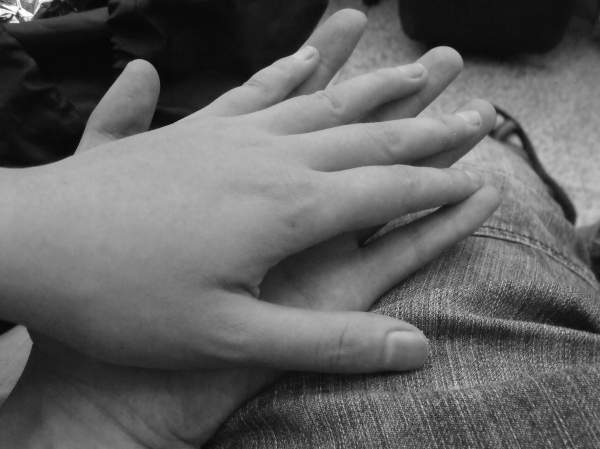
\includegraphics[width=0.6\textwidth]{images/hand_in_hand.png}}
\caption[]{\label{fig:hand_in_hand} 手拉手}
\end{figure}

\subsection{pgf/tikz绘图测试}
图\ref{fig:monotonic_chain}是用pgf/tikz宏包作的图形,用以说明计算几何相关定理。

\begin{figure}
\centering
\begin{tikzpicture}[line width=2pt]
\draw (-1,0) -- (8,0);
\draw (0,-1) -- (0,8);
\draw[step=.5cm, very thin] (0,0) grid (7.2,7.2);

\coordinate [label=above:$A$] (A) at (1, 4);
\coordinate [label=left:$B$] (B) at (0.5, 3.5);
\coordinate [label=left:$C$] (C) at (1, 3);
\coordinate [label=left:$D$] (D) at (0.3, 1.3);
\coordinate [label=below:$E$] (E) at (1, 1);

\draw[blue] (A) -- (B) -- (C)  -- (D) -- (E);
\draw[blue] (2, 0) -- (2, 6);

\coordinate [label=right:$A'$] (A') at (2, 4);
\coordinate [label=right:$B'$] (B') at (2, 3.5);
\coordinate [label=right:$C'$] (C') at (2, 3);
\coordinate [label=right:$D'$] (D') at (2, 1.3);
\coordinate [label=right:$E'$] (E') at (2, 1);

\draw[blue] (A) -- (A');
\draw[blue] (B) -- (B');
\draw[blue] (C) -- (C');
\draw[blue] (D) -- (D');
\draw[blue] (E) -- (E');

\coordinate [label=above:$a$] (a) at (5, 4);
\coordinate [label=left:$b$] (b) at (4.5, 4.5);
\coordinate [label=left:$c$] (c) at (5, 3);
\coordinate [label=left:$d$] (d) at (4.3, 1.3);
\coordinate [label=below:$e$] (e) at (5, 1.3);

\draw[green] (a) -- (b) -- (c)  -- (d) -- (e);
\draw[green] (6, 0) -- (6, 6);

\coordinate [label=right:$a'$] (a') at (6, 4);
\coordinate [label=right:$b'$] (b') at (6, 4.5);
\coordinate [label=right:$c'$] (c') at (6, 3);
\coordinate [label=right:$d'$] (d') at (6, 1.3);
\coordinate [label=right:$e'$] (e') at (6, 1.3);

\draw[green] (a) -- (a');
\draw[green] (b) -- (b');
\draw[green] (c) -- (c');
\draw[green] (d) -- (d');
\draw[green] (e) -- (e');
\end{tikzpicture}
\caption{Monotonic polygonal chains}
\label{fig:monotonic_chain}
\end{figure}

\section{表格测试}
\begin{table}[htbp]
  \centering
  \begin{tabular}[htbp]{r|l}
    \toprule
    日期 & 任务 \\
    \midrule
    2011.5 & 完善此份文档 \\
    2011.6 & 完善安装脚本 \\
    \bottomrule
  \end{tabular}
  \caption{表格}
  \label{tab:table1}
\end{table}

\section{源代码高亮测试}

以下是\href{http://acm.zju.edu.cn/onlinejudge/showProblem.do?problemCode=1372}{ZOJ 1372}的解题c++代码:

\begin{lstlisting}[language=c++]
#include <iostream>
#include <string>
using namespace std;
 
const long max_points = 100;
const long infinity = 1000001;
 
int p, r, length, g[max_points][max_points];
bool flag;
 
class vertex
{
public:
    int distance;
    bool visited;
};
 
vertex v[max_points];
 
void initial()
{
    for(int i = 1; i <= p; i++)
        for(int j = 1; j <= p; j++)
            g[i][j] = infinity;
}
 
void prim(int origin)
{
    int temp_min;
    int temp_v = 0;
    int sum = 0;
 
    for(int i = 1; i <= p; i++)
    {
        v[i].distance = g[i][origin];
        v[i].visited = false;
    }
 
    v[origin].distance = 0;
    v[origin].visited = true;
 
    sum++;
 
    while (sum < p)
    {
        temp_min = infinity;
        for(int i = 1; i <= p; i++)
            if(v[i].visited == false && v[i].distance < temp_min)
            {
                temp_min = v[i].distance;
                temp_v = i;
            }
         
        if(temp_min < infinity)
        {
            length += v[temp_v].distance;
            v[temp_v].visited = true;
            sum++;
        }
        else
        {
            flag = true;
            break;
        }
 
        for(int i = 1; i <= p; i++)
        {
            if(v[i].visited == false && v[i].distance > g[i][temp_v])
            {
                v[i].distance = g[i][temp_v];
            }
        }
    }
}
 
int main(int argc, char *argv[])
{
    int a, b, c;
 
    while(cin >> p)
    {
        if(p == 0)
            break;
        cin >> r;
 
        initial();
 
        for(int i = 0; i < r; i++)
        {
            cin >> a >> b >> c;
            if(c < g[a][b])
                g[a][b] = g[b][a] = c;
        }
        length = 0;
        prim(1);
 
        cout << length << endl;
    }
 
    return 0;
} 
\end{lstlisting}

\section{数学公式测试}

著名的爱因斯坦质能方程(\ref{eq:emc2}):

\begin{equation}
  \label{eq:emc2}
  E=mc^2
\end{equation}

计算$f(x)=x^2$的不定积分(\ref{eq:2}):

\begin{equation}
  \label{eq:2}
  \int x^2 dx = \frac{1}{3} x^3
\end{equation}
\section{参考文件测试}
参考文件最好使用bibtex,关于bibtex的使用方法,你可以自行查阅相关文献。

这里是参考文献\cite{c_minigui}

%%%%%%%%%------------------------------------------------------------------------
%%%% 附录

% \appendix    
% \appendixpage
%% 将附录条目添加到contents
% \addappheadtotoc

%%%% 附录结束
%%%%%%%%------------------------------------------------------------------------

%
%%% 加入参考文献支持
%\bibliography{data/main}
%%% 解决目录中没有相应的参考文献的条目问题
%\addcontentsline{toc}{section}{\refname} 
\end{document}
%%%% 正文部分结束
%%%%%%%%------------------------------------------------------------------------
